% Provenance (never printed): see sources/outline_sources.md (Year 2: sedimentary basins;
% subsidence curves and backstripping; the stretching model). Stretching model after McKenzie
% (1978) as restated by Sheplev and Reverdatto (1998) and coded in pyBacktrack (EarthByte);
% backstripping after pyBacktrack's well module; North Sea after Sclater and Christie (1980);
% Michigan after Sloss (1982) and Crowe et al. (2009); the US Atlantic margin after Schlee et
% al. (1976), Poag (1979) and Lang et al. (2024); the Molasse after the chapter 13 rows.
% Curves and the invented well from figdata/bachelor-2/basins.py; exercise and problem values
% in the Book 4 scratch calculator calc/ch16.py.
\chapter{Bacias sedimentares comparadas}\label{ch:b2:basins-compared}

Ao largo da costa leste dos Estados Unidos, sob a plataforma continental, o Baltimore
Canyon Trough contém pelo menos \qty{14}{km} de rocha sedimentar. Um poço perfurado numa tal
pilha lê sua história de trás para a frente: cada unidade que ele atravessa foi um dia o fundo do mar, a uma profundidade que
fósseis e sedimentos registram, e desde então foi soterrada e comprimida. A profundidade de cada
superfície datada é um ponto numa curva de afundamento. No entanto, a maior parte do afundamento foi causada pelo
peso do próprio sedimento. Para saber o que fez a bacia, esse peso tem de ser retirado,
camada por camada. Este capítulo mostra como, e o que o resultado diz sobre a litosfera.
% ledger: poag79:bct, schlee76:atlantic

\begin{recall}
\textbf{Do volume do primeiro ano}: bacia sedimentar, subsidência e subsidência tectônica,
acomodação, eustasia; compactação, descompactação e lei de Athy, a espessura sólida de uma
camada; a carga sedimentar, que amplifica a subsidência por $(\rho_m - \rho_w)/(\rho_m - \rho_s)$;
a isostasia de Airy; a litosfera e sua geoterma; os riftes continentais e as margens passivas.
\textbf{Dos volumes de física}: a equação do calor e suas soluções de Fourier.
\textbf{Do \cref{ch:b2:alpine-orogen}}: a \omterm{def:b2:alpine-orogen:foreland}{bacia de antepaís}, o \omterm{def:b2:alpine-orogen:foreland}{flysch} e a \omterm{def:b2:alpine-orogen:foreland}{molassa}.
\end{recall}

\begin{omfigure}
\centering
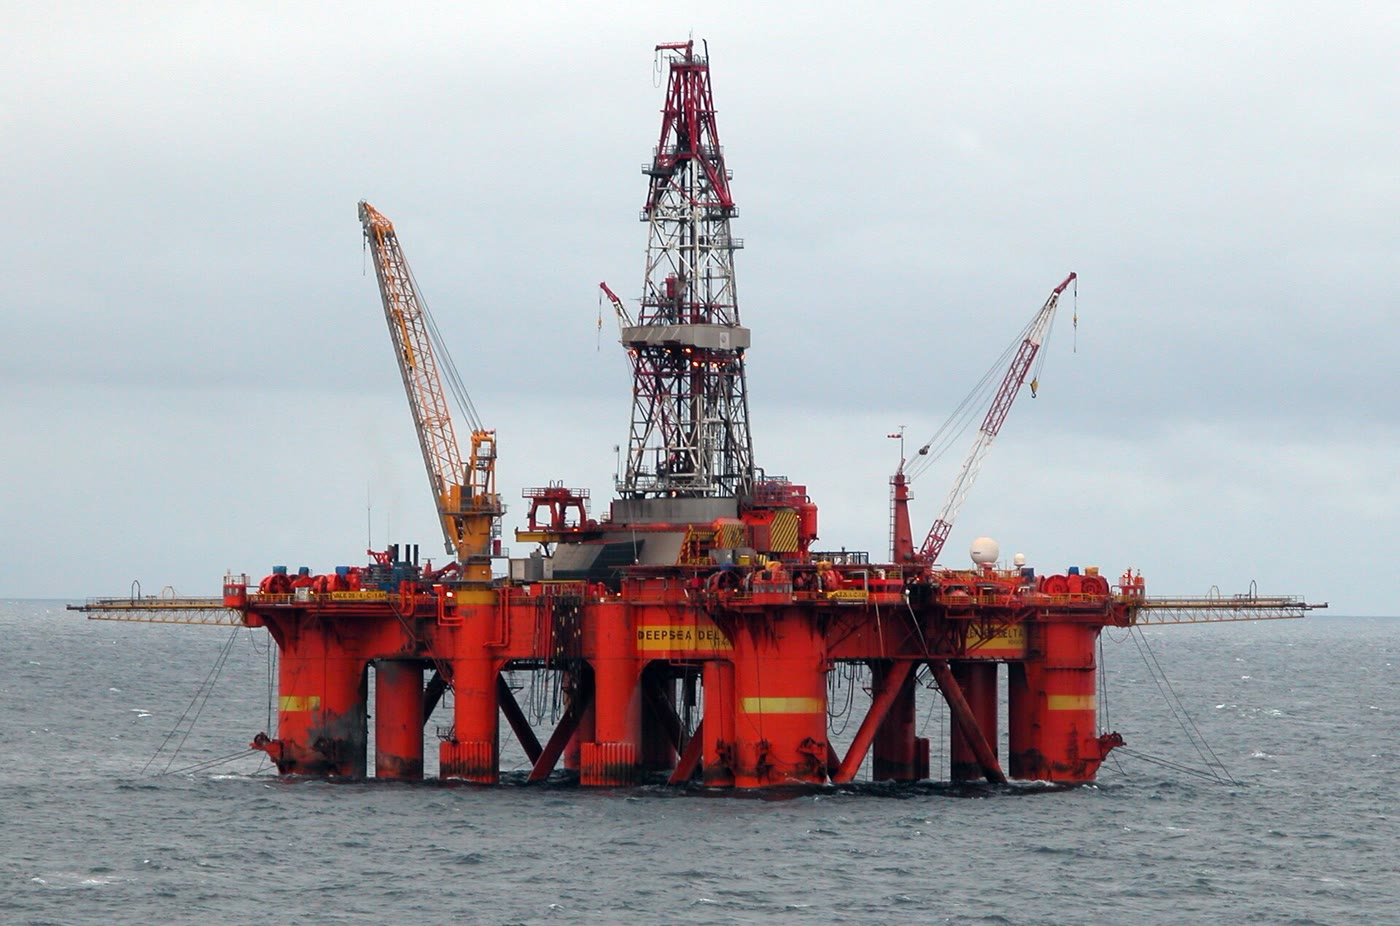
\includegraphics[width=0.66\linewidth]{images/book4/b2-16-drilling-rig.jpg}
\par\smallskip{\small Uma plataforma de perfuração semissubmersível no mar do Norte. Os poços perfurados
a partir dessas plataformas dão as espessuras, as idades e os tipos de rocha a partir dos quais a subsidência de uma bacia
é reconstruída. Fotografia de Erik Christensen, 2005, CC BY-SA 3.0.}
\end{omfigure}

\section{As bacias e o que as faz afundar}\label{sec:b2:basins-compared:types}

O volume do primeiro ano distinguia as bacias pelo lugar onde ficam. Aqui elas são distinguidas pelo que move
sua subsidência.

\begin{definition}[Bacias intracratônicas, de rifte e de margem passiva]\label{def:b2:basins-compared:types}
Uma \emph{bacia intracratônica}\index{bacia intracratônica} é uma bacia ampla, redonda ou oval, no
interior de um continente, longe dos limites de placas, que subside lentamente durante tempos muito longos
sem grandes falhamentos. Uma \emph{bacia de rifte}\index{bacia de rifte} é uma bacia limitada por falhas normais
numa litosfera continental em estiramento; sua subsidência acompanha o estiramento e depois
o resfriamento da litosfera. Uma \emph{bacia de margem passiva}\index{bacia de margem passiva} é a
cunha de sedimento, que se espessa em direção ao oceano, acumulada numa margem continental depois da
ruptura, sobre a crosta afinada do antigo rifte.
\end{definition}

A \omterm{def:b2:alpine-orogen:foreland}{bacia de antepaís} do \cref{ch:b2:alpine-orogen} completa a lista, e as bacias que se abrem
ao longo de falhas transcorrentes ficam para o volume do terceiro ano. Três mecanismos fazem o fundo de uma
bacia afundar:
\begin{itemize}
  \item o afinamento \emph{mecânico}: quando a crosta é estirada e afinada por falhas, crosta leve
        é substituída por manto mais denso e a superfície desce para restabelecer a isostasia;
  \item a contração \emph{térmica}: uma litosfera que foi aquecida, por estiramento ou por
        baixo, resfria-se depois, torna-se mais densa e afunda, lentamente, ao longo de dezenas de milhões de anos;
  \item a \emph{carga}: o peso de um cinturão de cavalgamentos, ou do próprio sedimento, curva a
        litosfera para baixo; essa flexão pertence ao volume do terceiro ano, e a forma local, de Airy, da
        carga sedimentar basta aqui.
\end{itemize}
As \omterm{def:b2:basins-compared:types}{bacias de rifte} combinam os dois primeiros, as margens passivas herdam o segundo de sua fase de rifte, e as
\omterm{def:b2:alpine-orogen:foreland}{bacias de antepaís} são feitas pelo terceiro. As \omterm{def:b2:basins-compared:types}{bacias intracratônicas} são as menos compreendidas.

\begin{omfigure}
\centering
\begin{tikzpicture}[x=1cm, y=1cm, font=\scriptsize, line join=round,
  sed/.style={fill=yellow!35, draw=black!60, line width=0.3pt},
  crust/.style={fill=orange!25, draw=black!60, line width=0.3pt},
  mlith/.style={fill=green!12, draw=black!60, line width=0.3pt},
  asth/.style={fill=red!12, draw=black!60, line width=0.3pt},
  sea/.style={fill=blue!8, draw=none},
  ttl/.style={anchor=south west, font=\scriptsize\bfseries}]
% (a) intracratonic
\begin{scope}
\fill[asth] (0,-2.4) rectangle (6.6,-1.6);
\fill[mlith] (0,-1.6) rectangle (6.6,-0.7);
\fill[crust] (0,-0.7) -- (6.6,-0.7) -- (6.6,0) -- (4.9,0) .. controls (4.1,-0.45) and (2.5,-0.45) .. (1.7,0) -- (0,0) -- cycle;
\fill[sed] (1.7,0) .. controls (2.5,-0.45) and (4.1,-0.45) .. (4.9,0) -- cycle;
\draw[black!70] (0,0) -- (6.6,0);
\node[ttl] at (0,0.05) {(a) intracratônica};
\node at (3.3,-1.15) {manto litosférico};
\node at (3.3,-2.0) {astenosfera};
\end{scope}
% (b) rift
\begin{scope}[xshift=7.2cm]
\fill[asth] (0,-2.4) -- (6.6,-2.4) -- (6.6,-1.6) -- (4.5,-1.6) -- (3.3,-1.0) -- (2.1,-1.6) -- (0,-1.6) -- cycle;
\fill[mlith] (0,-1.6) -- (2.1,-1.6) -- (3.3,-1.0) -- (4.5,-1.6) -- (6.6,-1.6) -- (6.6,-0.7) -- (4.4,-0.7) -- (3.3,-0.45) -- (2.2,-0.7) -- (0,-0.7) -- cycle;
\fill[crust] (0,-0.7) -- (2.2,-0.7) -- (3.3,-0.45) -- (4.4,-0.7) -- (6.6,-0.7) -- (6.6,0) -- (4.6,0) -- (4.25,-0.42) -- (3.75,-0.2) -- (3.35,-0.4) -- (2.95,-0.15) -- (2.45,-0.42) -- (2.0,0) -- (0,0) -- cycle;
\fill[sed] (2.0,0) -- (2.45,-0.42) -- (2.95,-0.15) -- (3.35,-0.4) -- (3.75,-0.2) -- (4.25,-0.42) -- (4.6,0) -- cycle;
\draw[thick] (2.0,0) -- (2.5,-0.5) (4.6,0) -- (4.2,-0.5) (2.95,-0.15) -- (3.4,-0.48);
\draw[black!70] (0,0) -- (6.6,0);
\node[ttl] at (0,0.05) {(b) rifte};
\node at (1.45,-1.15) {manto litosférico};
\node at (5.4,-2.0) {astenosfera};
\end{scope}
% (c) passive margin
\begin{scope}[yshift=-3.3cm]
\fill[asth] (0,-2.4) -- (6.6,-2.4) -- (6.6,-1.2) -- (0,-1.6) -- cycle;
\fill[mlith] (0,-1.6) -- (6.6,-1.2) -- (6.6,-1.0) -- (4.2,-1.05) -- (2.4,-0.75) -- (0,-0.7) -- cycle;
\fill[crust] (0,-0.7) -- (2.4,-0.75) -- (4.2,-1.05) -- (4.2,-0.85) -- (2.6,-0.25) -- (1.6,0) -- (0,0) -- cycle;
\fill[gray!35, draw=black!60, line width=0.3pt] (4.2,-1.05) -- (6.6,-1.0) -- (6.6,-0.85) -- (4.2,-0.85) -- cycle;
\fill[sed] (1.6,0) -- (2.6,-0.25) -- (4.2,-0.85) -- (6.6,-0.85) -- (6.6,-0.55) -- (3.6,-0.45) -- (2.6,-0.05) -- (2.2,0) -- cycle;
\fill[sea] (2.2,0) -- (6.6,0) -- (6.6,-0.55) -- (3.6,-0.45) -- (2.6,-0.05) -- cycle;
\draw[black!70] (0,0) -- (2.2,0);
\draw[blue!60!black] (2.2,0) -- (6.6,0);
\node[ttl] at (0,0.05) {(c) margem passiva};
\node at (5.4,-0.95) {\tiny crosta oceânica};
\node at (1.3,-2.0) {astenosfera};
\node at (1.3,-1.05) {manto litosférico};
\end{scope}
% (d) foreland
\begin{scope}[xshift=7.2cm, yshift=-3.3cm]
\fill[asth] (0,-2.4) -- (6.6,-2.4) -- (6.6,-2.0) -- (0,-1.5) -- cycle;
\fill[mlith] (0,-1.5) -- (6.6,-2.0) -- (6.6,-1.2) -- (0,-0.7) -- cycle;
\fill[crust] (0,-0.7) -- (6.6,-1.2) -- (6.6,-0.55) -- (3.6,-0.4) .. controls (2.0,-0.15) .. (0,0) -- cycle;
\fill[sed] (0,0) .. controls (2.0,-0.15) .. (3.6,-0.4) -- (6.6,-0.55) -- (5.0,0) -- cycle;
\fill[crust, fill=orange!45] (5.0,0) -- (6.6,-0.55) -- (6.6,0.6) -- (6.1,0.6) -- cycle;
\draw[thrust fault] (6.6,-0.55) -- (5.0,0);
\draw[black!70] (0,0) -- (5.0,0);
\node[ttl] at (0,0.05) {(d) antepaís};
\node[anchor=north east, font=\tiny] at (6.55,0.55) {cinturão};
\node at (2.2,-1.25) {manto litosférico};
\node at (1.5,-2.05) {astenosfera};
\end{scope}
\end{tikzpicture}
\par\smallskip{\small Quatro famílias de bacias em seções esquemáticas através da litosfera (fora
de escala; sedimento em amarelo, crosta continental em laranja, crosta oceânica em cinza). O exagero
vertical é grande: as bacias reais têm centenas de quilômetros de largura e de alguns a quinze
quilômetros de profundidade.}
\end{omfigure}

As \omterm{def:b2:basins-compared:types}{bacias de rifte} do mar do Norte são o caso clássico dos dois primeiros mecanismos. Grábens
se formaram ali a partir do Triássico, e o último grande estiramento durou do Jurássico Médio
a meados do Cretáceo; as falhas então se aquietaram, e o meio da bacia continuou afundando
como um amplo pires, preenchido por gizes, arenitos e, durante a maior parte do Terciário, folhelhos e
lamitos. Carregado só por água, seu embasamento teria afundado mais 1100 a
\qty{1400}{m} no meio e 600 a \qty{700}{m} nos flancos depois que o falhamento cessou.
% ledger: sc80b4:north-sea

A margem passiva do leste dos Estados Unidos mostra o mesmo afundamento numa escala maior.
Perfis sísmicos através da plataforma mostram mais de \qty{14}{km} de rocha mesozoica e mais jovem no
Baltimore Canyon Trough e \qty{8}{km} na bacia de Georges Bank, em unidades que se espessam
em direção ao oceano. Seus depocentros jurássicos seguem as estruturas do rifte e as zonas de sua
posterior subsidência térmica.
% ledger: schlee76:atlantic, lang24:atlantic

A bacia de Michigan é o tipo das \omterm{def:b2:basins-compared:types}{bacias intracratônicas}. Ovalada, com algumas centenas de milhares
de quilômetros quadrados de área, ela contém mais de \qty{4}{km} de sedimento fanerozoico depositado
em episódios distintos ao longo de uns 500 milhões de anos, com pouco falhamento. Seus episódios de subsidência
mais rápida coincidem com os de outras bacias nos interiores da América do Norte e de outros
continentes, o que sugere uma causa maior que uma bacia. O \omterm{def:b2:basins-compared:backstripping}{backstripping} de mais de 57\,000
perfis de poço mostra um padrão de subsidência duradouro, quase circular, que os autores sugerem
poder ser explicado por uma descida do manto, interrompido nas épocas de duas orogenias na distante
margem do continente. Por que as \omterm{def:b2:basins-compared:types}{bacias intracratônicas} afundam ainda é debatido.
% ledger: sloss82:michigan, crowe09:michigan

\section{Curvas de subsidência}\label{sec:b2:basins-compared:curves}

Um poço, ou uma seção medida, dá para cada unidade sua profundidade atual, seu tipo de rocha e sua idade,
lida nos fósseis ou por correlação. Com a profundidade da água na qual cada unidade foi
depositada, lida em seus fósseis e estruturas sedimentares, ele dá a história da bacia.

\begin{definition}[Curva de subsidência]\label{def:b2:basins-compared:curve}
Uma \emph{curva de subsidência}\index{curva de subsidência} de uma bacia num local é o gráfico da profundidade
de uma superfície de referência, geralmente o embasamento ou a base da unidade mais antiga, abaixo do nível do mar,
em função do tempo. A curva de subsidência \emph{total} usa a espessura do sedimento tal como era em cada
momento, mais a profundidade da água; a curva de subsidência \emph{tectônica} substitui o sedimento por água
e remove seu efeito isostático.
\end{definition}

Uma unidade nunca foi tão espessa no passado quanto é hoje. Soterrada, ela perdeu porosidade; seus grãos não
mudaram, mas sua água foi expulsa. O volume do primeiro ano escreveu a porosidade à profundidade
$z$ como a lei de Athy, $\phi(z) = \phi_0\,e^{-z/c}$, e encontrou a espessura sólida de uma camada entre
$z_1$ e $z_2$,
\[
  T_s = (z_2 - z_1) - \phi_0 c\left(e^{-z_1/c} - e^{-z_2/c}\right),
\]
que permanece a mesma quando a camada se desloca. Para \emph{descompactar} uma unidade até uma posição mais rasa,
com seu topo agora em $z_1'$, procura-se a base $z_2'$ que contém a mesma espessura sólida. A
equação não tem solução fechada, mas a iteração de ponto fixo
\[
  z_2' \leftarrow z_1' + T_s + \phi_0 c\left(e^{-z_1'/c} - e^{-z_2'/c}\right)
\]
a partir de $z_2' = z_1' + T_s$ converge em poucos passos. A massa por unidade de área da camada
é a de seus grãos mais a de sua água intersticial,
\[
  m = \rho_g T_s + \rho_w\,(z_2 - z_1 - T_s),
\]
sendo $\rho_g$ a densidade dos grãos; dividir a massa de uma coluna por sua espessura dá
sua densidade média $\bar\rho_s$.

Para as litologias usadas neste capítulo, areia, folhelho, giz e areia argilosa, a tabela abaixo
dá as constantes de Sclater e Christie (1980), tal como incluídas num programa de código aberto.
A areia conserva sua porosidade até mais fundo, o giz a perde mais depressa.
% ledger: pybacktrack:compaction

\begin{center}
\small
\begin{tabular}{lccc}
\hline
litologia & densidade dos grãos (\unit{kg.m^{-3}}) & porosidade superficial $\phi_0$ & escala de decaimento $c$ (\unit{m}) \\
\hline
areia & 2650 & 0.49 & 3704 \\
folhelho & 2700 & 0.63 & 1960 \\
giz & 2710 & 0.70 & 1408 \\
areia argilosa & 2680 & 0.56 & 2564 \\
\hline
\end{tabular}
\end{center}

\section{O backstripping}\label{sec:b2:basins-compared:backstripping}

Uma \omterm{def:b2:basins-compared:curve}{curva de subsidência} total mistura duas causas: o que quer que tenha feito a bacia, e o peso do que
a preencheu. Separá-las é o objetivo do procedimento seguinte, a ferramenta central da análise
de bacias.

\begin{definition}[Backstripping]\label{def:b2:basins-compared:backstripping}
O \emph{backstripping}\index{backstripping} é a reconstrução da subsidência tectônica de uma
bacia ao longo do tempo: as unidades de um poço são removidas uma a uma, a partir da mais jovem, as
restantes são descompactadas a cada passo, e o efeito isostático da carga de sedimento e de água
é removido para dar a profundidade em que o embasamento estaria sob água apenas.
\end{definition}

O último passo é um balanço isostático. O volume do primeiro ano o fez para uma bacia preenchida até o nível do mar;
o caso geral acrescenta a profundidade da água e o nível do mar.

\begin{proposition}[Backstripping de Airy]\label{prop:b2:basins-compared:backstrip}
Suponha-se que uma bacia contenha, num dado momento, uma coluna de sedimento de espessura $S$ e densidade média
$\bar\rho_s$, sob uma profundidade de água $W_d$, enquanto o mar estava $\Delta_{SL}$ acima do seu nível
atual. Em isostasia local sobre um manto de densidade $\rho_m$, com água de densidade $\rho_w$, a
subsidência tectônica nesse momento, medida a partir do nível do mar atual, é
\[
  Y = S\,\frac{\rho_m - \bar\rho_s}{\rho_m - \rho_w} + W_d
      - \Delta_{SL}\,\frac{\rho_m}{\rho_m - \rho_w}.
\]
\end{proposition}

\begin{proof}
Comparem-se duas colunas sobre a mesma litosfera, até uma profundidade de compensação abaixo das duas. Na
primeira, água de profundidade $W_d$ fica sobre o sedimento de espessura $S$; na segunda, só a água
preenche uma bacia de profundidade $Y'$ abaixo da mesma superfície do mar. Suas massas são iguais:
\[
  \rho_w W_d + \bar\rho_s S + \rho_m\,(d - W_d - S) = \rho_w Y' + \rho_m\,(d - Y'),
\]
sendo $d$ a profundidade comum do nível de compensação abaixo da superfície do mar. Logo
$Y'(\rho_m - \rho_w) = S(\rho_m - \bar\rho_s) + W_d(\rho_m - \rho_w)$, que são os dois primeiros
termos. Se o mar estava $\Delta_{SL}$ mais alto que hoje, essa água extra não faz parte da
subsidência própria da bacia: retirando-a, o embasamento carregado por água sobe de
$\Delta_{SL}\rho_w/(\rho_m - \rho_w)$, e sua profundidade abaixo do nível do mar atual diminui ainda de
$\Delta_{SL}$; juntos, $\Delta_{SL}\,\rho_m/(\rho_m - \rho_w)$.
\end{proof}
% ledger: pybacktrack:backstrip

Com $\rho_m = \qty{3330}{kg.m^{-3}}$ e $\rho_w = \qty{1030}{kg.m^{-3}}$, uma coluna de sedimento de
densidade média \qty{2300}{kg.m^{-3}} conta por $1030/2300 = 0.45$ de sua espessura na subsidência
tectônica: mais da metade da espessura do preenchimento de uma bacia é criada por seu próprio peso.
Um mar \qty{100}{m} mais alto que hoje reduz o resultado em \qty{145}{m}. A profundidade da água e o
nível do mar passado são os dados mais fracos: os fósseis dão um intervalo de profundidades de água, muitas vezes com centenas de
metros de amplitude no talude, e a subsidência tectônica herda esse intervalo.

\begin{method}[Backstripping de um poço]\label{met:b2:basins-compared:backstrip}
\begin{enumerate}
  \item Listem-se as unidades a partir da base, com as profundidades atuais de seus topos e bases, suas
        constantes litológicas $(\rho_g, \phi_0, c)$, as idades de seus topos e a profundidade da água em
        cada uma dessas idades.
  \item Calcule-se a espessura sólida $T_s$ de cada unidade a partir de suas profundidades atuais.
  \item Para a idade do topo da unidade $k$, removam-se todas as unidades mais jovens. Ponha-se o topo da unidade
        $k$ à profundidade zero e descompacte-se; ponha-se cada unidade mais antiga, por sua vez, sob a de cima
        e descompacte-se.
  \item Somem-se as espessuras para obter $S$, e as massas para obter a densidade média
        $\bar\rho_s = \sum m / S$.
  \item Aplique-se a \cref{prop:b2:basins-compared:backstrip} para obter $Y$; a subsidência total é
        $S + W_d$.
  \item Repita-se para cada idade, da mais antiga à atual; plotem-se $Y$ e $S + W_d$ em função da idade.
\end{enumerate}
\end{method}

A figura abaixo mostra o resultado para um poço inventado numa \omterm{def:b2:basins-compared:types}{bacia de rifte}. Quatro unidades foram testemunhadas:
uma areia sin-rifte depositada enquanto as falhas estavam ativas, entre 165 e \qty{150}{Ma}; depois um folhelho,
um giz e uma areia argilosa. Hoje, nenhuma descompactação é necessária: o embasamento está a \qty{6030}{m}
e a coluna tem uma densidade média de \qty{2358}{kg.m^{-3}}, de modo que $Y = \qty{2648}{m}$ sob
\qty{100}{m} de água. A \qty{150}{Ma}, a areia sozinha, descompactada na superfície, tinha
\qty{2239}{m} de espessura, com uma densidade média de \qty{2055}{kg.m^{-3}}: sob \qty{200}{m} de água,
$Y = \qty{1441}{m}$. A subsidência total é
mais que o dobro da tectônica, e a curva tectônica mostra uma primeira fase rápida, depois um
afundamento que se desacelera: a forma de um rifte.
% values (script): figdata/bachelor-2/basins.py part numbers (S_150 2239.5, rho_0 2357.9, Y_0 2648.7, Y_150 1442.1); printed from the rounded chain of calc/ch16.py (rho 2358 -> 2648; T 2239, rho 2055 -> 1441), as in the problem

\begin{omfigure}
\centering
% figdata/bachelor-2/basins.py parts stages and fit (invented well)
\begin{tikzpicture}
\begin{axis}[width=0.8\linewidth, height=6.0cm, x dir=reverse, y dir=reverse, xmin=0, xmax=170,
  ymin=0, ymax=6500, xlabel={idade (\unit{Ma})}, ylabel={profundidade abaixo do nível do mar (\unit{m})},
  tick label style={font=\scriptsize}, label style={font=\small}, xtick={0,25,...,175},
  xtick pos=bottom, ytick pos=left,
  legend style={at={(0.5,1.04)}, anchor=south, draw=none, font=\scriptsize, legend columns=3,
  /tikz/every even column/.append style={column sep=8pt}}]
\addplot[omThm, line width=1pt, mark=*, mark size=1.6pt] table[x=age_Ma, y=total_m]
  {figdata/out/bachelor-2-basins-stages.dat};
\addlegendentry{subsidência total $S + W_d$}
\addplot[blue!70!black, line width=1pt, mark=square*, mark size=1.6pt] table[x=age_Ma, y=Y_m]
  {figdata/out/bachelor-2-basins-stages.dat};
\addlegendentry{subsidência tectônica $Y$}
\addplot[black!70, dashed, line width=0.8pt] table[x=age_Ma, y=Y_m]
  {figdata/out/bachelor-2-basins-fit.dat};
\addlegendentry{modelo de estiramento, $\beta = 1.50$}
\node[font=\scriptsize, anchor=south west] at (axis cs:149,1500) {fim do rifteamento};
\end{axis}
\end{tikzpicture}
\par\smallskip{\small \omterm{def:b2:basins-compared:backstripping}{Backstripping} de um poço inventado com quatro unidades (dados no problema
de fim de semana): profundidade do embasamento com o sedimento tal como era em cada momento, e subsidência tectônica,
com a curva do \omterm{def:b2:basins-compared:stretching}{modelo de estiramento} ajustada à subsidência no fim do rifteamento
(\cref{sec:b2:basins-compared:stretching}).}
\end{omfigure}

\begin{omfigure}
\centering
\begin{tikzpicture}[x=1cm, y=0.1cm, font=\scriptsize, line join=round,
  u/.style={draw=black!60, line width=0.3pt}]
% today
\begin{scope}
\fill[blue!8] (0,0) rectangle (1.6,-1.0);
\fill[u, fill=yellow!25] (0,-1.0) rectangle (1.6,-18.0);
\fill[u, fill=green!18] (0,-18.0) rectangle (1.6,-34.1);
\fill[u, fill=gray!25] (0,-34.1) rectangle (1.6,-45.2);
\fill[u, fill=yellow!55] (0,-45.2) rectangle (1.6,-61.3);
\draw[black!70] (0,-61.3) -- (1.6,-61.3);
\node[anchor=south] at (0.8,0.1) {hoje};
\node at (0.8,-9.5) {areia argilosa};
\node at (0.8,-26) {giz};
\node at (0.8,-39.6) {folhelho};
\node at (0.8,-53.2) {areia};
\node[anchor=north] at (0.8,-61.5) {\qty{6130}{m}};
\end{scope}
% at 150 Ma
\begin{scope}[xshift=3.0cm]
\fill[blue!8] (0,0) rectangle (1.6,-2.0);
\fill[u, fill=yellow!55] (0,-2.0) rectangle (1.6,-24.39);
\draw[black!70] (0,-24.4) -- (1.6,-24.4);
\node[anchor=south] at (0.8,0.1) {\qty{150}{Ma}};
\node at (0.8,-13.2) {areia};
\node[anchor=north] at (0.8,-24.6) {\qty{2439}{m}};
\end{scope}
\draw[-{Latex}, thick] (4.9,-12) -- (6.1,-12) node[midway, above] {descarregar};
% water loaded
\begin{scope}[xshift=6.3cm]
\fill[blue!20] (0,0) rectangle (1.6,-14.4);
\draw[black!70] (0,-14.4) -- (1.6,-14.4);
\node[anchor=south] at (0.8,0.1) {só água};
\node at (0.8,-7.2) {água};
\node[anchor=north] at (0.8,-14.6) {$Y = \qty{1441}{m}$};
\end{scope}
\draw[black!40, dashed] (-0.3,0) -- (8.2,0);
\node[anchor=west] at (8.2,0) {nível do mar};
\end{tikzpicture}
\par\smallskip{\small \omterm{def:b2:basins-compared:backstripping}{Backstripping} do poço inventado a \qty{150}{Ma} (profundidades em escala): as
quatro unidades hoje; a areia sozinha no fim do rifteamento, descompactada na superfície sob
\qty{200}{m} de água; a mesma litosfera carregada só por água, cujo embasamento fica
mais alto porque a água é mais leve que o sedimento.}
\end{omfigure}

\section{O modelo de estiramento}\label{sec:b2:basins-compared:stretching}

Por que uma \omterm{def:b2:basins-compared:types}{bacia de rifte} afunda primeiro depressa e depois devagar? Em 1978, D. McKenzie propôs um modelo tão
simples que seus parâmetros podem ser ajustados a um único poço.

\begin{definition}[Modelo de estiramento; fator de estiramento; subsidência sin-rifte e pós-rifte]\label{def:b2:basins-compared:stretching}
O \emph{modelo de estiramento}\index{modelo de estiramento} de uma bacia representa o rifteamento como um
estiramento instantâneo e uniforme de toda a litosfera por cisalhamento puro: crosta e manto
litosférico são afinados pelo mesmo fator, e a astenosfera quente sobe passivamente para preencher o
espaço, depois do que a litosfera se resfria. O \emph{fator de estiramento}\index{fator de estiramento}
$\beta$ é a razão entre a largura da região estirada depois do estiramento e sua largura antes,
igual à razão entre a espessura inicial e a final da crosta. A subsidência produzida
durante o estiramento é a \emph{subsidência sin-rifte}\index{subsidência sin-rifte}; a produzida
depois pelo resfriamento da litosfera é a \emph{subsidência
pós-rifte}\index{subsidência pós-rifte}, ou subsidência térmica.
\end{definition}

O estiramento na natureza leva um tempo finito, milhões de anos. Versões posteriores do modelo o deixam
durar, mas, desde que não seja lento demais, a versão instantânea simples dá a subsidência
de forma aproximada mas correta, pois depois do estiramento o resfriamento procede quase da mesma maneira.
% ledger: sheplev98:model

\begin{omfigure}
\centering
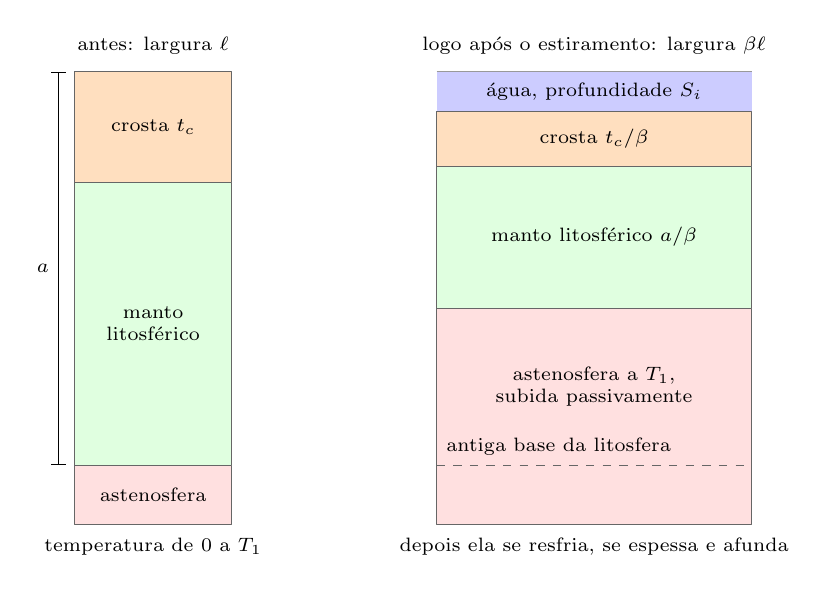
\begin{tikzpicture}[x=0.5cm, y=0.5cm, font=\scriptsize, line join=round]
% before
\begin{scope}
\fill[orange!25, draw=black!60, line width=0.3pt] (0,0) rectangle (4,-2.8);
\fill[green!12, draw=black!60, line width=0.3pt] (0,-2.8) rectangle (4,-10);
\fill[red!12, draw=black!60, line width=0.3pt] (0,-10) rectangle (4,-11.5);
\node at (2,-1.4) {crosta $t_c$};
\node[align=center] at (2,-6.4) {manto\\litosférico};
\node at (2,-10.75) {astenosfera};
\draw[|-|] (-0.4,0) -- (-0.4,-10) node[midway, left] {$a$};
\node[anchor=south] at (2,0.2) {antes: largura $\ell$};
\node[anchor=north] at (2,-11.6) {temperatura de $0$ a $T_1$};
\end{scope}
% after
\begin{scope}[xshift=4.6cm]
\fill[blue!20] (0,0) rectangle (8,-1.0);
\fill[orange!25, draw=black!60, line width=0.3pt] (0,-1.0) rectangle (8,-2.4);
\fill[green!12, draw=black!60, line width=0.3pt] (0,-2.4) rectangle (8,-6.0);
\fill[red!12, draw=black!60, line width=0.3pt] (0,-6.0) rectangle (8,-11.5);
\draw[black!60, dashed] (0,-10) -- (8,-10);
\node at (4,-0.5) {água, profundidade $S_i$};
\node at (4,-1.7) {crosta $t_c/\beta$};
\node at (4,-4.2) {manto litosférico $a/\beta$};
\node[align=center] at (4,-8.0) {astenosfera a $T_1$,\\subida passivamente};
\node[anchor=south west] at (0,-10) {antiga base da litosfera};
\node[anchor=south] at (4,0.2) {logo após o estiramento: largura $\beta\ell$};
\node[anchor=north] at (4,-11.6) {depois ela se resfria, se espessa e afunda};
\draw[black!40] (0,0) -- (8,0);
\end{scope}
\end{tikzpicture}
\par\smallskip{\small O \omterm{def:b2:basins-compared:stretching}{modelo de estiramento} (fora de escala): uma litosfera de espessura $a$ com uma
crosta $t_c$ é estirada até $\beta$ vezes sua largura; crosta e manto litosférico se afinam por
$\beta$, a astenosfera sobe, e a superfície afunda da \omterm{def:b2:basins-compared:stretching}{subsidência sin-rifte} $S_i$ sob
água. Aqui $\beta = 2$.}
\end{omfigure}

\begin{proposition}[Subsidência no modelo de estiramento]\label{prop:b2:basins-compared:stretching}
Considere-se uma litosfera de espessura $a$, com uma crosta de espessura $t_c$, uma geoterma linear de
$0$ na superfície até a temperatura $T_1$ da astenosfera em sua base; sejam as densidades da crosta e do manto
$\rho_c(1 - \alpha T)$ e $\rho_m(1 - \alpha T)$, sendo $\alpha$ o coeficiente de
dilatação térmica. Se ela é estirada instantaneamente por $\beta$ e a bacia preenchida com
água de densidade $\rho_w$:
\begin{enumerate}
  \item a \omterm{def:b2:basins-compared:stretching}{subsidência sin-rifte} é
  \[
    S_i = \frac{a\left(1 - \dfrac{1}{\beta}\right)\left[(\rho_m - \rho_c)\dfrac{t_c}{a}
          \left(1 - \dfrac{\alpha T_1 t_c}{2a}\right) - \dfrac{\alpha T_1 \rho_m}{2}\right]}
          {\rho_m(1 - \alpha T_1) - \rho_w};
  \]
  \item a \omterm{def:b2:basins-compared:stretching}{subsidência pós-rifte}, um tempo $t$ depois do estiramento, é, no primeiro termo de uma série,
  \[
    S_t = E_0\,\frac{\beta}{\pi}\sin\frac{\pi}{\beta}\left(1 - e^{-t/\tau}\right),\qquad
    E_0 = \frac{4a\rho_m\alpha T_1}{\pi^2(\rho_m - \rho_w)},\qquad
    \tau = \frac{a^2}{\pi^2\kappa},
  \]
  onde $\kappa$ é a difusividade térmica e $\tau$ é a \emph{constante de tempo
  térmica}\index{constante de tempo térmica} da litosfera.
\end{enumerate}
\end{proposition}
% ledger: pybacktrack:rifting

\begin{proof}
(1) Compare-se a coluna antes do estiramento com a coluna logo depois, até a antiga base da
litosfera, à profundidade $a$ abaixo da superfície antes do estiramento. Antes, a crosta de
espessura $t_c$ e o manto litosférico estão às temperaturas $T = T_1 z/a$; depois, ambos estão
mais finos por $\beta$ e suas temperaturas vão de $0$ a $T_1$ ao longo de $a/\beta$, de modo que um ponto
à profundidade $z'$ abaixo da base da água tem $T = T_1\beta z'/a$; abaixo, a astenosfera a
$T_1$ tem densidade $\rho_m(1 - \alpha T_1)$; acima, a água preenche a profundidade $S_i$. A massa de uma
camada de densidade $\rho(1 - \alpha T)$ na qual $T$ cresce linearmente de $T_a$ a $T_b$ é
$\rho\,h\,(1 - \alpha(T_a + T_b)/2)$. Antes, a coluna contém
\[
  \rho_c t_c\left(1 - \frac{\alpha T_1 t_c}{2a}\right)
  + \rho_m (a - t_c)\left(1 - \frac{\alpha T_1 (a + t_c)}{2a}\right);
\]
depois, ela contém a água, a crosta e o manto litosférico afinados, e a astenosfera que
preenche o resto da profundidade $a$:
\[
  \rho_w S_i + \frac{\rho_c t_c}{\beta}\left(1 - \frac{\alpha T_1 t_c}{2a}\right)
  + \frac{\rho_m (a - t_c)}{\beta}\left(1 - \frac{\alpha T_1 (a + t_c)}{2a}\right)
  + \rho_m(1 - \alpha T_1)\left(a - S_i - \frac{a}{\beta}\right).
\]
A isostasia torna as duas iguais. Reunindo os termos em $S_i$ de um lado e o fator
$(1 - 1/\beta)$ do outro, e desenvolvendo, obtém-se a fórmula; a álgebra é o
\cref{exo:b2:basins-compared:11}.

(2) Depois do estiramento, a placa se resfria por condução entre uma superfície mantida a $0$ e uma base mantida
a $T_1$, em direção ao perfil linear do qual partiu. O excesso de temperatura satisfaz a equação do
calor com valores nulos no topo e na base, e é portanto uma soma de termos
$b_n\sin(n\pi z/a)\,e^{-n^2\kappa\pi^2 t/a^2}$; cada um se resfria com seu próprio tempo, $\tau/n^2$. O
calor perdido faz a coluna se contrair de $\alpha\int \Delta T\,\mathrm{d}z$, e a água extra
que preenche o espaço a faz afundar mais pelo fator $\rho_m/(\rho_m - \rho_w)$. Só os termos ímpares
contribuem; conservar o primeiro, cujo coeficiente é calculado a partir do perfil inicial, dá
a expressão. Os outros se resfriam nove ou mais vezes mais depressa, e depois de cerca de dez milhões de anos
deslocam a subsidência de uma quantidade quase constante, menor que \qty{100}{m} para $\beta$ de
1.2 a 4 com os valores abaixo.
\end{proof}
% values (script): basins.thermal_series vs basins.thermal, tested in tests/bachelor-2/test_basins.py

Os parâmetros do artigo de McKenzie são $a = \qty{125}{km}$, $T_1 = \qty{1333}{\celsius}$,
$\alpha = \qty{3.28e-5}{K^{-1}}$, $\kappa = \qty{8e-7}{m^2.s^{-1}}$, $\rho_m =
\qty{3330}{kg.m^{-3}}$ (a \qty{0}{\celsius}), $\rho_c = \qty{2800}{kg.m^{-3}}$; com água do mar a
\qty{1030}{kg.m^{-3}}, eles dão $\tau = \qty{62.7}{Myr}$ e $E_0 = \qty{3207}{m}$. Com uma crosta de
\qty{35}{km}, a \omterm{def:b2:basins-compared:stretching}{subsidência sin-rifte} é $S_i = \qty{4334}{m} \times (1 - 1/\beta)$.
% ledger: sheplev98:parameters, pybacktrack:rifting
% values (script): tau_Myr 62.7, E0_m 3206.9, Si_max_m 4333.8

\begin{omfigure}
\centering
% figdata/bachelor-2/basins.py part curves
\begin{tikzpicture}
\begin{axis}[width=0.8\linewidth, height=6.2cm, y dir=reverse, xmin=0, xmax=200, ymin=0,
  ymax=6500, xlabel={tempo depois do estiramento (\unit{Myr})},
  ylabel={subsidência tectônica (\unit{m})}, tick label style={font=\scriptsize},
  label style={font=\small}, xtick pos=bottom, ytick pos=left]
\addplot[black!45, line width=1pt] table[x=t_Myr, y=b1.2] {figdata/out/bachelor-2-basins-curves.dat};
\addplot[blue!70!black, line width=1pt] table[x=t_Myr, y=b1.5] {figdata/out/bachelor-2-basins-curves.dat};
\addplot[omThm, line width=1pt] table[x=t_Myr, y=b2] {figdata/out/bachelor-2-basins-curves.dat};
\addplot[orange!80!black, line width=1pt] table[x=t_Myr, y=b4] {figdata/out/bachelor-2-basins-curves.dat};
\node[font=\scriptsize, anchor=south west, inner sep=1pt] at (axis cs:150,1225) {$\beta = 1.2$};
\node[font=\scriptsize, anchor=south west, inner sep=1pt] at (axis cs:150,2595) {$\beta = 1.5$};
\node[font=\scriptsize, anchor=south west, inner sep=1pt] at (axis cs:150,3965) {$\beta = 2$};
\node[font=\scriptsize, anchor=south west, inner sep=1pt] at (axis cs:150,5815) {$\beta = 4$};
\draw[black!40, dashed] (axis cs:62.7,0) -- (axis cs:62.7,6500);
\node[font=\scriptsize, anchor=north west] at (axis cs:63,150) {$t = \tau$};
\end{axis}
\end{tikzpicture}
\par\smallskip{\small Subsidência carregada por água do \omterm{def:b2:basins-compared:stretching}{modelo de estiramento} para quatro \omterm{def:b2:basins-compared:stretching}{fatores de
estiramento}, com uma crosta de \qty{35}{km} e os parâmetros do texto: o degrau sin-rifte em
$t = 0$, depois a curva pós-rifte, que atingiu \qty{63}{\percent} do seu valor final em
$t = \tau$.}
\end{omfigure}

Três traços do modelo se transferem para as bacias reais.
\begin{itemize}
  \item O degrau sin-rifte cresce com $\beta$, e a \omterm{def:b2:basins-compared:stretching}{subsidência pós-rifte} também; mas sua
        razão muda pouco, de modo que as duas partes apontam para o mesmo $\beta$ se o modelo vale.
  \item A escala de tempo da \omterm{def:b2:basins-compared:stretching}{subsidência pós-rifte} não depende de $\beta$: ela é fixada apenas pela
        espessura da litosfera. Depois de $\tau$, \qty{63}{\percent} da subsidência
        térmica está feita; depois de $3\tau$, cerca de \qty{95}{\percent}. Um rifte que parou há duzentos
        milhões de anos quase não afunda mais.
  \item O termo sin-rifte é uma competição entre a crosta leve afinada, que faz a
        superfície afundar, e a astenosfera quente que subiu, que a faz flutuar. Com uma crosta fina, a
        segunda vence e o estiramento eleva a superfície (\cref{exo:b2:basins-compared:10}).
\end{itemize}

Para ajustar um poço, a subsidência tectônica no fim do rifteamento dá $S_i$, logo
$\beta = 1/(1 - S_i/\qty{4334}{m})$ para uma crosta de \qty{35}{km}; a curva pós-rifte é então prevista
e comparada com o resto dos pontos obtidos por \omterm{def:b2:basins-compared:backstripping}{backstripping}. No poço inventado, $S_i = \qty{1441}{m}$
dá $\beta = 1.50$, e a curva passa a poucos metros dos pontos posteriores (figura na
\cref{sec:b2:basins-compared:backstripping}). As bacias reais raramente são tão complacentes. No
mar do Norte central, um estiramento de 50 a \qty{100}{\percent} no meio, $\beta$ de 1.5 a 2,
reproduz a amplitude e a taxa da \omterm{def:b2:basins-compared:stretching}{subsidência pós-rifte}. Na margem do leste dos
Estados Unidos, só um segmento, a Long Island Platform, tem um preenchimento pós-rifte inicial tão espesso
quanto prevê o estiramento uniforme; na Georges Bank Basin e no Baltimore Canyon Trough, o
preenchimento é de 1.5 a 3 vezes mais espesso, e outras causas devem estar atuando.
% ledger: sc80b4:north-sea, lang24:atlantic

\section{Bacias comparadas}\label{sec:b2:basins-compared:compared}

A tabela abaixo reúne as quatro famílias. As curvas diferem em forma e em escala de tempo, e uma
\omterm{def:b2:basins-compared:curve}{curva de subsidência} é muitas vezes a primeira pista sobre a natureza de uma bacia soterrada sob rochas mais jovens.

\begin{center}
\small
\begin{tabular}{>{\raggedright\arraybackslash}p{0.13\linewidth}>{\raggedright\arraybackslash}p{0.19\linewidth}>{\raggedright\arraybackslash}p{0.26\linewidth}>{\raggedright\arraybackslash}p{0.29\linewidth}}
\hline
bacia & exemplo & espessura e duração & forma da \omterm{def:b2:basins-compared:curve}{curva de subsidência} tectônica \\
\hline
rifte & mar do Norte central & grábens a partir do Triássico; último estiramento do Jurássico Médio a
meados do Cretáceo; 1.1 a \qty{1.4}{km} de afundamento pós-rifte carregado por água & um degrau sin-rifte rápido,
depois uma desaceleração exponencial com $\tau$ de dezenas de Myr \\
margem passiva & Baltimore Canyon Trough & mais de \qty{14}{km} desde o Jurássico & como um
rifte, com uma grande parte pós-rifte; o preenchimento se espessa em direção ao oceano \\
antepaís & \omterm{def:b2:alpine-orogen:foreland}{Molassa} do norte dos Alpes & mais de \qty{4}{km} na frente de cavalgamento, do Eoceno Superior ao
Mioceno Superior & mais profunda junto ao cinturão e migrando com ele; sua parte interna é por fim
cavalgada pelos cavalgamentos \\
intracratônica & Michigan & mais de \qty{4}{km} em episódios ao longo de uns 500 Myr & lenta, com
episódios de afundamento mais rápido compartilhados por bacias distantes \\
\hline
\end{tabular}
\end{center}
% ledger: sc80b4:north-sea, schlee76:atlantic, poag79:bct, krenmayr99:molasse, schmid04:foreland, sloss82:michigan

Uma \omterm{def:b2:alpine-orogen:foreland}{bacia de antepaís} afunda sob uma carga que se move em sua direção: a bacia migra com o cinturão,
a alpina por pelo menos \qty{210}{km} sobre o cráton europeu, e sua parte interna é
por fim cavalgada e transportada pelos cavalgamentos, como a \omterm{def:b2:alpine-orogen:foreland}{Molassa} Subalpina foi no
\cref{ch:b2:alpine-orogen}. Um rifte se desacelera à medida que se resfria, qualquer que seja
seu estiramento. Uma \omterm{def:b2:basins-compared:types}{bacia intracratônica} afunda devagar e por muito tempo, em pulsos; nem o estiramento
nem uma carga a explicam bem, e é por isso que ela continua sendo uma questão de pesquisa.
% ledger: schmid04:foreland, sinclair97:trinity, krenmayr99:molasse

\begin{inthelab}[Análise de subsidência]
Os analistas de bacias fazem o trabalho do quadro de método com programas. Um programa de código aberto, por
exemplo, lê um poço como uma lista de unidades com suas idades, profundidades e litologias, e uma
tabela de litologias com sua densidade dos grãos, porosidade superficial e escala de decaimento. Seu
módulo de \omterm{def:b2:basins-compared:backstripping}{backstripping} descompacta as unidades e devolve a subsidência tectônica em cada idade;
como uma paleoprofundidade da água só é conhecida como um intervalo, o usuário dá um mínimo e um máximo e
o programa devolve as duas subsidências e sua média. Um segundo módulo funciona no sentido inverso:
a partir de um modelo de subsidência tectônica, ele prevê as profundidades de água do passado, que podem ser
conferidas com os fósseis. Os analistas então ajustam \omterm{def:b2:basins-compared:stretching}{fatores de estiramento}, testam curvas do nível do mar, e
mapeiam a subsidência de uma bacia inteira a partir de centenas ou milhares de poços.
\end{inthelab}
% ledger: pybacktrack:modules, crowe09:michigan

\section*{Exercícios}\label{sec:b2:basins-compared:exercises}

Dados para os exercícios, salvo indicação contrária: $\rho_m = \qty{3330}{kg.m^{-3}}$, $\rho_c =
\qty{2800}{kg.m^{-3}}$, $\rho_w = \qty{1030}{kg.m^{-3}}$; \omterm{def:b2:basins-compared:stretching}{modelo de estiramento} com $a =
\qty{125}{km}$, $T_1 = \qty{1333}{\celsius}$, $\alpha = \qty{3.28e-5}{K^{-1}}$, $\kappa =
\qty{8e-7}{m^2.s^{-1}}$, $\tau = \qty{62.7}{Myr}$, $E_0 = \qty{3207}{m}$; uma crosta de \qty{35}{km}
dá $S_i = \qty{4334}{m}\times(1 - 1/\beta)$; constantes litológicas na tabela da
\cref{sec:b2:basins-compared:curves}.

\begin{exercise}[$\star$]\label{exo:b2:basins-compared:1}
Dê a família de cada bacia e a causa principal de sua subsidência: (a) a bacia de Michigan;
(b) o mar do Norte central; (c) o Baltimore Canyon Trough; (d) a \omterm{def:b2:alpine-orogen:foreland}{Molassa} do norte dos Alpes;
(e) a planície indo-gangética diante do Himalaia.
\end{exercise}

\begin{exercise}[$\star$]\label{exo:b2:basins-compared:2}
Uma bacia contém \qty{3.0}{km} de sedimento de densidade média \qty{2300}{kg.m^{-3}}. (a) Encontre sua
subsidência tectônica se o sedimento chega ao nível do mar. (b) E se \qty{200}{m} de água estiverem por
cima? (c) Que fração da espessura do preenchimento se deve à carga do próprio preenchimento?
\end{exercise}

\begin{exercise}[$\star$]\label{exo:b2:basins-compared:3}
A refração sísmica mostra que uma crosta de \qty{35}{km} foi afinada para \qty{25}{km} num rifte.
(a) Quanto vale $\beta$? (b) Que espessura tem a litosfera logo depois do estiramento? (c) Qual é a
\omterm{def:b2:basins-compared:stretching}{subsidência sin-rifte} sob água?
\end{exercise}

\begin{exercise}[$\star$]\label{exo:b2:basins-compared:4}
(a) Verifique que $\tau = \qty{62.7}{Myr}$ ($1~\text{Myr} = \qty{3.156e13}{s}$). (b) Alguns programas
usam $\kappa = \qty{1e-6}{m^2.s^{-1}}$: quanto vale então $\tau$? (c) Quanto valeria para uma
litosfera de \qty{100}{km} de espessura, com $\kappa = \qty{8e-7}{m^2.s^{-1}}$? (d) Que fração da
\omterm{def:b2:basins-compared:stretching}{subsidência pós-rifte} está feita depois de $\tau$, e depois de $3\tau$?
\end{exercise}

\begin{exercise}[$\star\star$]\label{exo:b2:basins-compared:5}
Uma unidade de folhelho está hoje entre \qty{1000}{m} e \qty{2000}{m}. (a) Encontre sua porosidade no
topo e na base. (b) Encontre sua espessura sólida. (c) Encontre sua massa por unidade de área e sua densidade
média, com os poros cheios de água.
\end{exercise}

\begin{exercise}[$\star\star$]\label{exo:b2:basins-compared:6}
O folhelho do \cref{exo:b2:basins-compared:5} é trazido de volta à superfície. (a) Itere a
fórmula de descompactação a partir de $z_2' = T_s$ até que ela mude menos de \qty{1}{m}. (b) Qual é
sua densidade média na superfície? (c) Quanto mais espesso ele era?
\end{exercise}

\begin{exercise}[$\star\star$]\label{exo:b2:basins-compared:7}
No mar do Norte central, o embasamento carregado por água afundou de 1100 a \qty{1400}{m} depois do
estiramento que terminou em meados do Cretáceo, há cerca de \qty{100}{Myr}. (a) Que \omterm{def:b2:basins-compared:stretching}{subsidência
pós-rifte} o modelo dá depois de \qty{100}{Myr} para $\beta = 1.5$ e $\beta = 2$? (b) Esses
valores enquadram a observação? (c) Para que $\beta$ o modelo dá \qty{1250}{m}?
Use $\frac{\beta}{\pi}\sin\frac{\pi}{\beta} = 0.4705$ para $\beta = 1.6$ e $0.5204$ para $\beta
= 1.7$ e interpole.
\end{exercise}

\begin{exercise}[$\star\star$]\label{exo:b2:basins-compared:8}
A bacia sin-rifte de um \omterm{def:b2:basins-compared:stretching}{modelo de estiramento} é preenchida não por água, mas por sedimento de densidade
\qty{2300}{kg.m^{-3}}. (a) Na fórmula de $S_i$, o que muda? (b) Calcule o $S_i$ carregado por sedimento
para $\beta = 1.5$ com uma crosta de \qty{35}{km}, sabendo que o numerador da fórmula é
$a(1 - 1/\beta)\times\qty{74.69}{kg.m^{-3}}$ e que $\rho_m(1 - \alpha T_1) =
\qty{3184.4}{kg.m^{-3}}$. (c) Compare com o valor carregado por água.
\end{exercise}

\begin{exercise}[$\star\star$]\label{exo:b2:basins-compared:9}
Um poço submetido a \omterm{def:b2:basins-compared:backstripping}{backstripping} dá $Y = \qty{2171}{m}$ a \qty{100}{Ma}, supondo o nível do mar atual. (a)
Se o mar estava então \qty{100}{m} mais alto, quanto vale $Y$? (b) Se os fósseis dão uma profundidade de água
entre 100 e \qty{500}{m} em vez de \qty{300}{m}, que intervalo de $Y$ resulta? (c) Qual das
duas incertezas é a maior?
\end{exercise}

\begin{exercise}[$\star\star\star$]\label{exo:b2:basins-compared:10}
(a) Mostre, a partir da \cref{prop:b2:basins-compared:stretching}, que o estiramento faz a superfície subir
em vez de afundar quando $(\rho_m - \rho_c)\frac{t_c}{a}\left(1 - \frac{\alpha T_1 t_c}{2a}\right) <
\frac{\alpha T_1\rho_m}{2}$. (b) Desprezando o termo pequeno $\alpha T_1 t_c/(2a)$, encontre a
espessura crustal crítica. (c) Refine-a com uma iteração. (d) Onde na Terra você procuraria
riftes que sobem enquanto se abrem?
\end{exercise}

\begin{exercise}[$\star\star\star$]\label{exo:b2:basins-compared:11}
(a) Escreva o balanço isostático da demonstração da \cref{prop:b2:basins-compared:stretching}, parte
(1), e deduza a fórmula de $S_i$. (b) Mostre que a \omterm{def:b2:basins-compared:stretching}{subsidência pós-rifte} final exata, quando
a placa voltou à sua geoterma linear, é $\alpha\rho_m T_1 a(1 - 1/\beta)/(2(\rho_m -
\rho_w))$. (c) Calcule-a para $\beta = 2$ e compare-a com o valor final da
fórmula do primeiro termo.
\end{exercise}

\begin{exercise}[$\star\star\star$]\label{exo:b2:basins-compared:12}
Uma margem passiva foi estirada por $\beta = 2$ e vem se resfriando há \qty{150}{Myr}; a
bacia permaneceu cheia de sedimento de densidade média \qty{2400}{kg.m^{-3}} até o nível do mar.
(a) Encontre a \omterm{def:b2:basins-compared:stretching}{subsidência pós-rifte} carregada por água. (b) Que espessura tem o sedimento pós-rifte?
(c) No Baltimore Canyon Trough, o preenchimento pós-rifte inicial é de 1.5 a 3 vezes mais espesso do que
prevê o estiramento uniforme: que espessura isso significaria aqui? (d) Sugira causas.
\end{exercise}

\begin{problem}[{Problema de fim de semana --- backstripping de um poço}]\label{pb:b2:basins-compared:1}
Na Bacia Kestrel, inventada, um poço testemunhou quatro unidades. A partir da base: uma areia depositada durante
o rifteamento, de 165 a \qty{150}{Ma}, hoje entre \qty{4420}{m} e \qty{6030}{m}; um folhelho, de 150
a \qty{100}{Ma}, entre \qty{3310}{m} e \qty{4420}{m}; um giz, de 100 a \qty{60}{Ma}, entre
\qty{1700}{m} e \qty{3310}{m}; uma areia argilosa, de \qty{60}{Ma} até hoje, entre \qty{0}{m} e
\qty{1700}{m} abaixo do fundo do mar. Os fósseis dão a profundidade da água no topo de cada unidade quando ela
foi depositada: \qty{200}{m} a \qty{150}{Ma}, \qty{300}{m} a \qty{100}{Ma}, \qty{150}{m} a
\qty{60}{Ma}; hoje ela é de \qty{100}{m}. Use a tabela de litologias do capítulo, $\rho_m =
\qty{3330}{kg.m^{-3}}$ e $\rho_w = \qty{1030}{kg.m^{-3}}$ tanto para a água do mar quanto para a água intersticial, o nível do mar
como hoje, e o \omterm{def:b2:basins-compared:stretching}{modelo de estiramento} do capítulo com uma crosta de \qty{35}{km}. As profundidades são arredondadas
ao metro.

\noindent\textbf{Parte I --- Compactação.}
\begin{enumerate}
  \item Encontre a porosidade da areia em seu topo e em sua base hoje.
  \item Encontre a espessura sólida da areia.
  \item As espessuras sólidas do folhelho, do giz e da areia argilosa são \qty{1011}{m},
        \qty{1409}{m} e \qty{1004}{m}. Confira uma delas.
  \item Encontre a massa por unidade de área de cada unidade hoje, depois a densidade média de toda a
        coluna.
  \item A \qty{150}{Ma}, a areia estava no fundo do mar. Descompacte-a: itere a partir de $z_2' =
        T_s$ até que a variação seja menor que \qty{1}{m}.
  \item Encontre a densidade média da areia descompactada.
\end{enumerate}

\noindent\textbf{Parte II --- Backstripping.}
\begin{enumerate}[resume]
  \item Encontre a subsidência tectônica $Y$ a \qty{150}{Ma}.
  \item Encontre a subsidência tectônica hoje. Por que nenhuma descompactação é necessária?
  \item Um programa dá $Y = \qty{2171}{m}$ a \qty{100}{Ma} e $Y = \qty{2453}{m}$ a
        \qty{60}{Ma}. Calcule a taxa média de subsidência tectônica em cada um dos três
        intervalos desde \qty{150}{Ma}.
  \item Encontre a subsidência total hoje e compare-a com a subsidência tectônica.
  \item Que fração da profundidade do embasamento hoje se deve à carga do sedimento?
  \item Se o mar a \qty{100}{Ma} estivesse \qty{100}{m} mais alto que hoje, quanto teria sido $Y$
        então?
\end{enumerate}

\noindent\textbf{Parte III --- Ajustar o modelo de estiramento.} O rifteamento é tomado como instantâneo
e terminando a \qty{150}{Ma}.
\begin{enumerate}[resume]
  \item Que ponto da curva dá a \omterm{def:b2:basins-compared:stretching}{subsidência sin-rifte}?
  \item Encontre o \omterm{def:b2:basins-compared:stretching}{fator de estiramento} $\beta$, com duas casas decimais.
  \item Que espessura tinham a crosta e a litosfera logo depois do estiramento?
  \item Com $\beta$ arredondado, calcule $\frac{\beta}{\pi}\sin\frac{\pi}{\beta}$ e a \omterm{def:b2:basins-compared:stretching}{subsidência
        pós-rifte} final.
  \item Preveja $Y$ a 100, 60 e \qty{0}{Ma}.
  \item Compare com os valores obtidos por \omterm{def:b2:basins-compared:backstripping}{backstripping}.
  \item O ajuste é bom porque o poço é inventado. Dê três razões pelas quais um poço real não
        se ajustaria tão bem.
\end{enumerate}

\noindent\textbf{Parte IV --- Os próximos 50 milhões de anos.}
\begin{enumerate}[resume]
  \item Quanta subsidência tectônica a mais ocorrerá nos próximos \qty{50}{Myr}?
  \item Se a profundidade da água permanecer em \qty{100}{m}, quanto sedimento de densidade
        \qty{2400}{kg.m^{-3}} pode se acumular nesse tempo?
  \item Que fração de sua \omterm{def:b2:basins-compared:stretching}{subsidência pós-rifte} final a bacia já realizou?
  \item Quando metade dela estava realizada?
  \item Para resumir: que \omterm{def:b2:basins-compared:stretching}{fator de estiramento} o poço registra?
\end{enumerate}
\end{problem}
